\section{Task 1: Normalisation}

Figure 1 below shows part of a spreadsheet used by a tavern which allows customers to book rooms for events and functions. Each row represents a booking.

\begin{figure}[H]
\centering
\caption{Tavern Bookings}
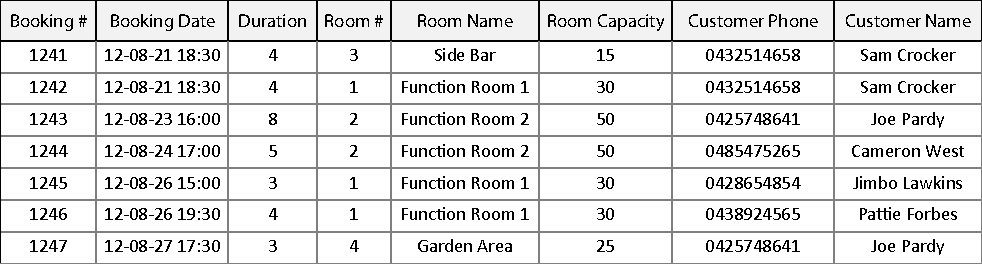
\includegraphics[scale=0.8]{./img/task1.pdf}
\end{figure}

\subsection{Assumptions}

\begin{itemize}
% \item The pub currently identifies customers by their phone number
\item A room cannot have multiple bookings at the same time
\item Auto-incrementing Customer\# has been created, replacing CustomerPhone as customer identifier
	\begin{itemize}
	\item Auto-incrementing identifier avoids user input error which may result in multiple customers with the same phone number
	\item Allows CustomerPhone to be updated without having to update foreign keys if CustomerPhone remained as identifier
	\end{itemize}
\item BookingDate time element has been split into its own attribute
	\begin{itemize}
	\item New attributes created called BookingTimeStart and BookingTimeEnd
	\item Duration attribute is now derived, no longer stored on database
	\item Allows system to check availability of room before a new booking can be created
	\end{itemize}
\end{itemize}

\subsection{0NF: Unnormalised form}

R1 = (Customer\#, CustomerPhone, CustomerName, {Booking\#, BookingDate, BookingTimeStart, BookingTimeEnd, Room\#, RoomName, RoomCapacity})

\subsection{1NF: First normal form}

\sout{R1 = (\textbf{\underline{Customer\#}}, CustomerPhone, CustomerName, \{\textbf{\underline{Booking\#}}, BookingDate, BookingTimeStart, BookingTimeEnd, Room\#,RoomName, RoomCapacity\})}
\\\\
R11 = (\textbf{\underline{Customer\#}}, CustomerPhone, CustomerName)
\\\\
R12 = (\textbf{\underline{Booking\#}}, BookingDate, BookingTimeStart, BookingTimeEnd, Room\#, RoomName, RoomCapacity, \emph{Customer\#})

\subsection{2NF: Second normal form}

No partial dependencies, already 2NF.
\\\\
R11 = (\textbf{\underline{Customer\#}}, CustomerPhone, CustomerName)
\\\\
R12 = (\textbf{\underline{Booking\#}}, BookingDate, BookingTimeStart, BookingTimeEnd, Room\#, RoomName, RoomCapacity, \emph{Customer\#})

\subsection{3NF: Third normal form}

R11 = (\textbf{\underline{Customer\#}}, CustomerPhone, CustomerName)
\\\\
\sout{R12 = (\textbf{\underline{Booking\#}}, BookingDate, BookingTimeStart, BookingTimeEnd, Room\#, RoomName, RoomCapacity, \emph{Customer\#})}
\\\\
R121 = (\textbf{\underline{Booking\#}}, BookingDate, BookingTimeStart, BookingTimeEnd, \emph{Room\#}, \emph{Customer\#})
\\\\
R122 = (\textbf{\underline{Room\#}}, RoomName, RoomCapacity)

\subsection{Named relations}

Customer = (\textbf{\underline{Customer\#}}, CustomerPhone, CustomerName)
\\\\
Booking = (\textbf{\underline{Booking\#}}, BookingDate, BookingTimeStart, BookingTimeEnd, \emph{Room\#}, \emph{Customer\#})
\\\\
Room = (\textbf{\underline{Room\#}}, RoomName, RoomCapacity)

\subsection{Physical E-R diagram}